\section{Introduction}


\paragraph{???} \st{Here I must be writing something really motivational.}
\\
% \cite{russakovsky2015imagenet} "In the last three years, mainly due to the advances of deep learning, more concretely convolutional networks, the quality of image recognition and object detection has been progressing at a dramatic pace".


\paragraph{Adversarial attack}
~\cite{DBLP:journals/corr/abs-1802-08195} "Goodfellow define adversarial examples as “inputs to machine learning models that an
attacker has intentionally designed to cause the model to make a mistake.” In the context of visual
object recognition, adversarial examples are images usually formed by applying a small perturbation
to a naturally occurring image in a way that breaks the predictions made by a machine learning
classifier".
\\
It’s widely known fact that NN are vulnerable against adversarial images.
\\\cite{ilyas2019adversarial} "Particularly worrisome is the phenomenon of adversarial examples, imperceptibly perturbed natural inputs that induce erroneous predictions in state-of-the-art classifiers."\newline

\paragraph{Pretext task}
The pretext task is the self-supervised learning task solved to learn visual representations,
with the aim of using the learned representations or model weights obtained in the process, for the downstream task.
As Alexander Kolesnikov and Xiaohua Zhai and Lucas Beyer~\cite{kolesnikov2019revisiting} have shown in their paper,
pretext tasks had proven to increase models accuracy, and are also believed to contribute to model learning important
(as per human agents) features.

\paragraph{Research question}
In this paper I would like to evaluate how state-of-the-art pretext \\
tasks influence NNs vulnerability against adversarial attacks.



\subsection{Background and Related work}
\paragraph{Efficient Net}
Convolutional networks' architectures for image recognition have evolved quite drastically in recent yers, with numerous options available "out of the box".
One which caught authors (my) eyes most recently was Efficient Net (further denoted as EffNet)\cite{DBLP:journals/corr/abs-1905-11946} as it delivers impressive accuracy, while being able to scale better than a lot of others and being not so resource greedy.
So, I would be using it alongside with own way simpler implementation to evaluate the research.

\paragraph{Rotation pretext training}
~\cite{kolesnikov2019revisiting} "Gidaris et al.propose to produce 4 copies of
a single image by rotating it by {0°, 90°, 180°, 270°} and let
a single network predict the rotation which was applied—a
4-class classification task.
Intuitively, a good model should learn to recognize canonical orientations of objects in natural images."

\paragraph{Jigsaw pretext training}
As described by described here~\cite{kolesnikov2019revisiting},
the task is to recover relative spatial position of
4 randomly sampled image patches after a random permutation of these patches was performed.
All of these patches are concatenated in 'puzzle' image, which is later sent through same network, which needs to predict a permutation that
was used.
In practice, 4 out of 24 possible permutations were used.

\paragraph{Fast gradient sign method}
This name was first introduced by Goodfellow and Jonathon Shlens and Christian Szegedy in their paper
~\cite{goodfellow2015explaining} as guaranteed approach to make artificial neural network miss-classify image,
which still would de be recognisable as of the same class for humans. \newline
The fast gradient sign method (further denoted as FGSM) works by using the gradients of the neural network to create an adversarial pattern.
For an input image, the method uses the gradients of the loss with respect to the input image to create a new image that maximises the loss.
This new image is called the adversarial image.
This can be summarised using the following expression: $adv\_x = x + \epsilon \cdot sign(\nabla_x J(\theta, x, y))$
\\ (where $\epsilon$ denotes the intensity of adversarial pattern).


\section{Methods}

\paragraph{Models}
The implementation was done using tensorflow framework using simple convolutional network and EfficientNet alogside.
Own basic implementation is based on \href{https://www.tensorflow.org/tutorials/images/classification}{Tensorflow image classification}.
For more details about EfficientNet usage, please refer to \href{https://keras.io/api/applications/efficientnet/}{Keras EfficientNet}.



\paragraph{Rotation pretext task}
Each image from original dataset was rotated 0°,90°,180°,270° and assigned new pseudo label in [0\ldots3].
New images were shuffled afterwards.
The last dense layer of network was replaced with dense layer for corresponding number of pseudo classes (4).
The same model was then trained to identify rotation applied.
\\
\begin{figure}[!htp]
    \begin{subfigure}{0.33\textwidth}
        \caption{Label = 0}
        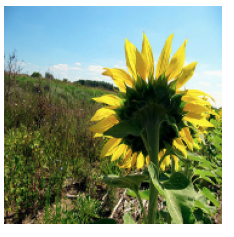
\includegraphics[width=5cm]{images/rot_0}
    \end{subfigure}
    \begin{subfigure}{0.2\textwidth}
        \caption{Label = 1}
        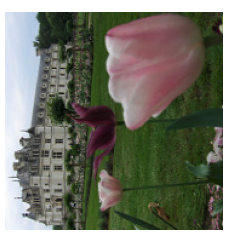
\includegraphics[width=5cm]{images/rot_1}
    \end{subfigure}
    \begin{subfigure}{0.33\textwidth}
        \caption{Label = 2}
        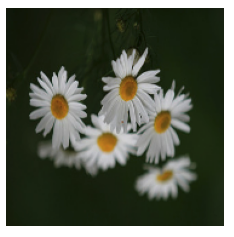
\includegraphics[width=5cm]{images/rot_2}
    \end{subfigure}
\end{figure}

\paragraph{Jigsaw pretext task}
For jigsaw I have adopted similar approach as described by Mehdi Noroozi and Paolo Favaro in their paper\cite{DBLP:journals/corr/NorooziF16}.
Image was cut in 4 equal parts, 4 out of 24 possible premutations were chosen for each batch.
(number of possible permutation can be obtained from Newtonian binomial $P=\frac{r!}{(r-n)!}$).
Similarly to rotation pseudo labels in [0\ldots23] have been assigned, data was shuffled and dense layer was replaced by suitable one.
The network then is trained to identify permutation applied.
\\
\begin{figure}
    \begin{subfigure}{0.33\textwidth}
        \caption{Original image}
        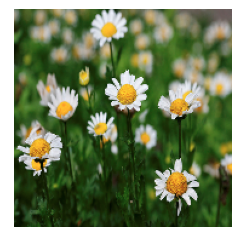
\includegraphics[width=5cm]{images/dandelion}
    \end{subfigure}
    \begin{subfigure}{0.2\textwidth}
        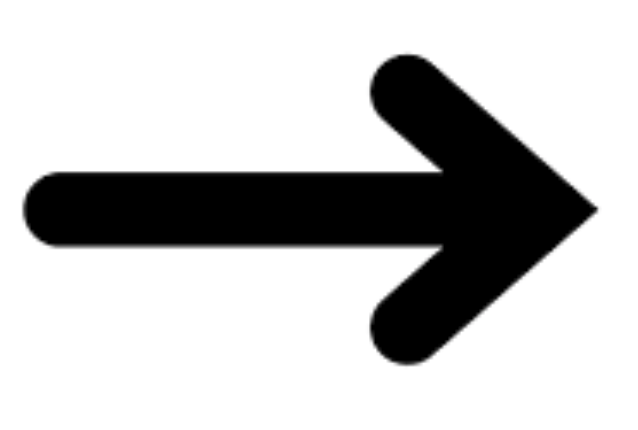
\includegraphics[width=3cm]{images/arrow}
    \end{subfigure}
    \begin{subfigure}{0.33\textwidth}
        \caption{Generated puzzle, with label=1}
        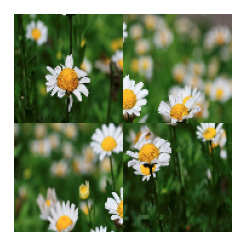
\includegraphics[width=5cm]{images/puzzle}
    \end{subfigure}
\end{figure}

\paragraph{Adversarial Images with FGSM}
My implementation of FGSM is based on \href{https://www.tensorflow.org/tutorials/generative/adversarial_fgsm}{TF FGSM}.
In order to generate adversarial pattern for each image, gradient of loss function is evaluated with sign for each image.
Then it's overlapped with original image with $\epsilon$ in [0.01, 0.1, 0.15], as any higher values make the image visually disrupted
for human viewer(like me).
\\
\begin{figure}[!h]
    \begin{subfigure}{0.33\textwidth}
        \caption{Labrador retriever 41.82\% confidence}
        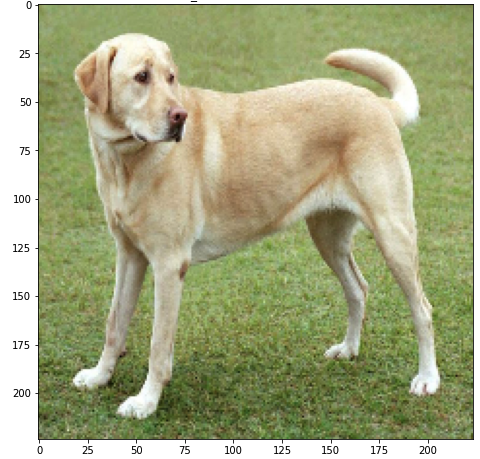
\includegraphics[width=5cm]{images/labrador}
    \end{subfigure}
    \begin{subfigure}{0.33\textwidth}
        \caption{Adversarial pattern}
        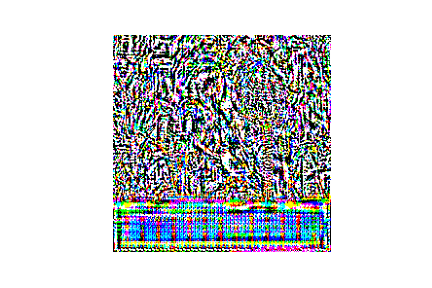
\includegraphics[width=5cm]{images/adv_pattern}
    \end{subfigure}
    \begin{subfigure}{0.3\textwidth}
        \caption{Weimaraner 15.13\% confidence}
        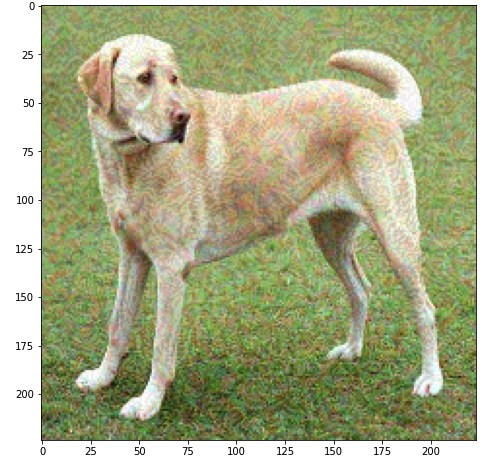
\includegraphics[width=5cm]{images/adv_labrador}
    \end{subfigure}
\end{figure}

\paragraph{Evaluation approach}
In order to evaluate, how including pretext task in training process influences NNs vulnerability against adversarial attacks,
I have measured intensity of adversarial pattern needed to make NN miss classify (Further denoted with epsilon or $\epsilon$).
\newline
5\% of dataset were reserved for experiment.
During each evaluation round NN network was trained with either none, rotation, jigsaw, or both, pretext tasks.
Number of training epochs was varied in [10, 20, 30, 50] for pretext and downstream task.
\\
Reserved images were \st{fed} to NN, the ones which were correctly classified saved.
Then each of saved (previously correctly classified images) was overlapped with adversarial pattern generated for it.
If classification was still correct $\epsilon$ value was increased.
\\
The smallest value needed to cause miss classification was saved.
$\overline{\epsilon}$ was compared for different values of pretext training epochs, downstream training epochs,
and kinds of pretext tasks.
\\
In order to compare how pretext tasks preform in comparison with other popular state of the art pre-training technics perform,
I will also compare EffNet trained with pretext tasks by myself with EffNet pre-trained on ImageNet utilized in transfer learning manner.